\chapter{Continual Learning and Foundation Models}
\label{ch:framework}

Continual Learning (CL) is the central problem this thesis addresses: how can a visual recognition system keep learning new object categories over time without catastrophically forgetting the ones it already knows? Answering this question rigorously, however, first requires a shared vocabulary. Before discussing what makes forgetting happen, what has been tried to prevent it, and how this thesis proposes to avoid it altogether, we must establish the fundamental principles of Artificial Intelligence, Machine Learning, and Deep Learning on which every subsequent argument rests, closing this introductory background with Computer Vision and its Object Classification task---the specific setting, including a first, necessarily brief, encounter with the Transformer architecture, in which the Continual Learning problem studied in this thesis is framed.

With this vocabulary in place, we return to Continual Learning and examine it in the depth the central problem of this thesis demands: the challenge of catastrophic forgetting, the stability--plasticity dilemma it creates, the main paradigms used to formulate it, and a review of the state-of-the-art mitigation strategies that provide both a performance baseline and the motivation for this thesis. This review then gives way, fluidly, to the representation-learning backbone that the proposed framework builds upon: Vision Transformers and, in particular, the self-supervised DINOv2 architecture.

\section{Artificial Intelligence and Machine Learning}
\label{sec:framework:ai_ml}

Artificial Intelligence (AI) is a broad field of computer science dedicated to creating systems capable of performing tasks that typically require human intelligence, such as learning, reasoning, perception, and language understanding \cite{RussellNorvig}. Within this domain, Machine Learning (ML) focuses on developing algorithms that allow computers to learn patterns from data without explicit programming. ML systems are generally categorized into three paradigms: Supervised Learning, Unsupervised Learning, and Reinforcement Learning \cite{Bishop2006}.

First, in \textbf{Supervised Learning}, the model learns a mapping from input variables $\mathbf{x}$ to output variables $y$ based on a labeled dataset $\mathcal{D} = \{(\mathbf{x}_i, y_i)\}_{i=1}^N$. The objective is to minimize a loss function that penalizes the discrepancy between the predicted output and the ground truth. This paradigm is typically divided into Classification, where the output is a discrete category, and Regression, where the output is a continuous value.

Second, \textbf{Unsupervised Learning} deals with unlabeled data $\mathcal{D} = \{\mathbf{x}_i\}_{i=1}^N$. Instead of predicting a target, the goal is to discover the underlying structure or distribution of the data. Common tasks include Clustering, which groups similar data points (e.g., K-Means or Gaussian Mixture Models), and Dimensionality Reduction, which projects high-dimensional data into a lower-dimensional space while preserving essential information (e.g., PCA or t-SNE).

Finally, \textbf{Reinforcement Learning} is based on an agent interacting with an environment to maximize a cumulative reward. Unlike supervised learning, the agent is not told which actions to take but must discover them through trial and error. This process is often modeled as a Markov Decision Process (MDP) \cite{Sutton2018}, where the agent transitions between states based on actions, receiving feedback in the form of numerical rewards. 
The focus is on finding an optimal policy that maximizes long-term return, a process that requires balancing exploration (trying new actions) and exploitation (capitalizing on known high-reward actions) during learning.
 %The focus is on finding an optimal policy that balances exploration (trying new actions) and exploitation (using known high-reward actions).

\subsection{Deep Learning}

In traditional Machine Learning, the feature extraction step is a manual process where a human expert must identify and define the most relevant characteristics (such as the shape or edges of the car) before passing them to a classification algorithm. In contrast, as shown in figure \ref{fig:deep_learning}, Deep Learning utilizes neural networks to automate this process; the model performs both feature extraction and classification simultaneously, learning to identify complex patterns directly from the input data without human intervention.

This shift allows Deep Learning to handle much more complex, high-dimensional data, though it typically requires significantly larger datasets and more computational power to be effective. While traditional Machine Learning depends on the quality of hand-crafted features, Deep Learning architectures—like multi-layered neural networks—are designed to build hierarchical representations of data, progressively moving from low-level pixels to high-level object concepts.

\begin{figure}[htb]
	\centering
	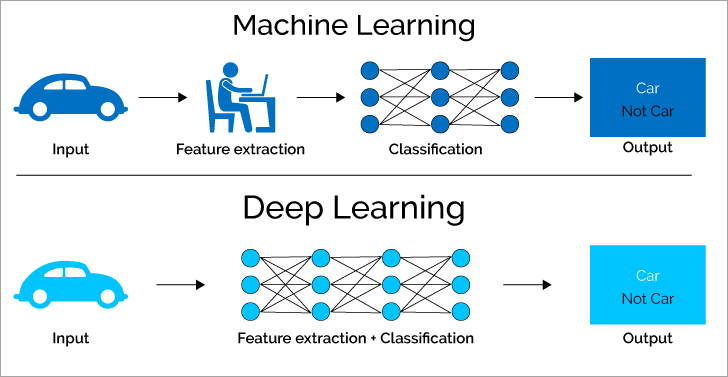
\includegraphics[width=0.7\textwidth]{imagenes/marco/deep.png}
	\caption{Machine Learning and Deep Learning Strategies. Image taken from \cite{deep}.}
	\label{fig:deep_learning}
\end{figure}

\subsection{Computer Vision}
\label{sec:framework:cv}

Computer Vision is the interdisciplinary field that enables computers to gain high-level understanding from digital images or videos, effectively automating tasks performed by the human visual system \cite{Szeliski2010}. While Convolutional Neural Networks (CNNs) \cite{CNN} historically dominated this field, the Transformer architecture---originally developed for Natural Language Processing---has revolutionized visual recognition through the self-attention mechanism \cite{AttentionIsAllYouNeed}.

Among the many tasks studied in Computer Vision, \textbf{Object Classification} is one of the most fundamental: it consists of assigning a single categorical label to an entire input image, and it serves as the primary benchmark for evaluating the representative power of visual models \cite{Krizhevsky2012}. This task is the setting adopted throughout this thesis: the Continual Learning problem discussed next is studied specifically as a sequence of object classification tasks, in which the model must progressively learn to assign incoming images to a growing set of object categories.

Having established this general background in Artificial Intelligence, Machine Learning, Deep Learning, and Computer Vision---including a first glimpse of the Transformer architecture that will reappear in depth later in this chapter---we now turn to the specific paradigm around which this thesis is organized: Continual Learning, studied here within the object classification setting.

\section{Continual Learning}
\label{sec:framework:cl}

Continual Learning (CL), also known as lifelong learning, addresses the problem of progressively acquiring knowledge from non-stationary data streams over time. In object classification, this setup presents data as a sequence of disjoint tasks, where each task introduces a new set of object categories. The primary challenge is enabling a model to learn these novel categories incrementally without degrading its classification performance on previously acquired ones. As illustrated in Figure \ref{fig:task_time}, a \textbf{task} in this context a is 
defined as a specific learning session or split—such as Task A, B, or C—each introducing distinct class-conditional data distributions, symbolized by the varying shapes (e.g., circles vs. hearts) above the task labels.

% is defined as a specific learning experience or dataset –such as Task A, B, or C. Each task is potentially characterized by unique data distributions or objectives, as symbolized by the varying shapes (e.g., circles vs. hearts) above the task labels.

Unlike conventional training approaches that rely on a fixed dataset and a stationary environment, CL emphasizes the arrival of these tasks at distinct intervals along the \textbf{time} axis. This sequential arrival requires the model to be inherently non-stationary, adapting its internal representations as environments evolve. The primary challenge in this paradigm lies in the ongoing integration of new information from a current task (e.g., Task B) while simultaneously preserving the knowledge previously acquired from Task A.

\begin{figure}[htb]
	\centering
	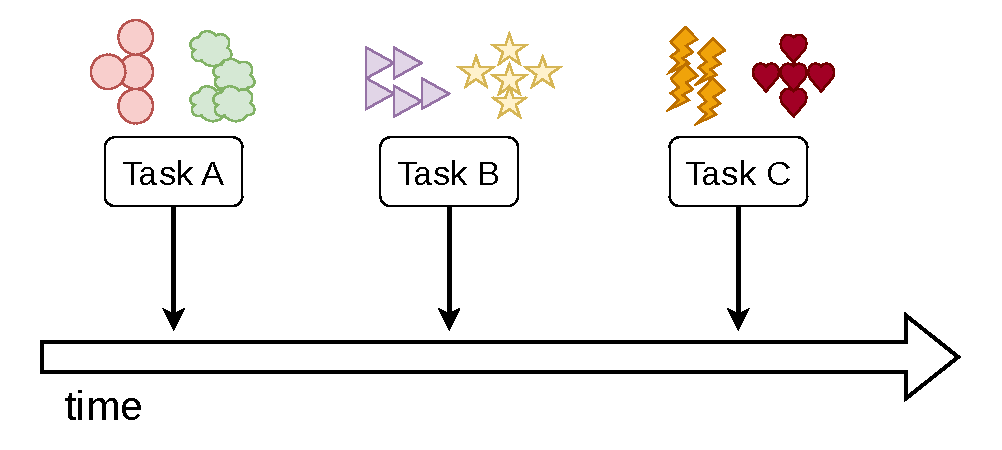
\includegraphics[width=0.75\textwidth]{imagenes/marco/Adaptation.pdf}
	\caption{A sequential task arrival model for Continual Learning, depicting the transition from Task A to Task C over time, where each task represents a unique set of features or data distributions.}
	\label{fig:task_time}
\end{figure}

Without specific architectural or algorithmic safeguards, this sequential learning process inevitably triggers \textbf{catastrophic forgetting} \cite{CL}. This phenomenon occurs when the assimilation of new knowledge leads to the degradation or total loss of prior learning. As illustrated in Figure \ref{fig:catastrophic_forgetting}, the dilemma of forgetting becomes apparent when a \textit{New Object Class} is introduced to an existing classifier, forcing a choice between two traditional but flawed strategies:

\begin{itemize}
	\item \textbf{Fine-Tuning:} Updating the model using only the current task data is computationally efficient but leads directly to catastrophic forgetting \cite{CL}. Because the optimization process focuses solely on the new objective, the internal representations associated with previously learned classes are overwritten, causing the model to lose its original predictive capabilities.

	\item \textbf{Retraining from Scratch:} While joint training on the full historical dataset ($\mathcal{D}_{old} \cup \mathcal{D}_{new}$) technically prevents forgetting, it faces two significant hurdles. First is the issue of \textbf{Data Privacy and Availability}: in many real-world scenarios, the original data $\mathcal{D}_{old}$ is often deleted or inaccessible due to privacy regulations. Second is the \textbf{Computational Bottleneck}: as the system's lifespan increases, the cumulative dataset grows, making the energy and time required to retrain the model unsustainable in continuously evolving environments.
\end{itemize}

\begin{figure}[htb]
	\centering
	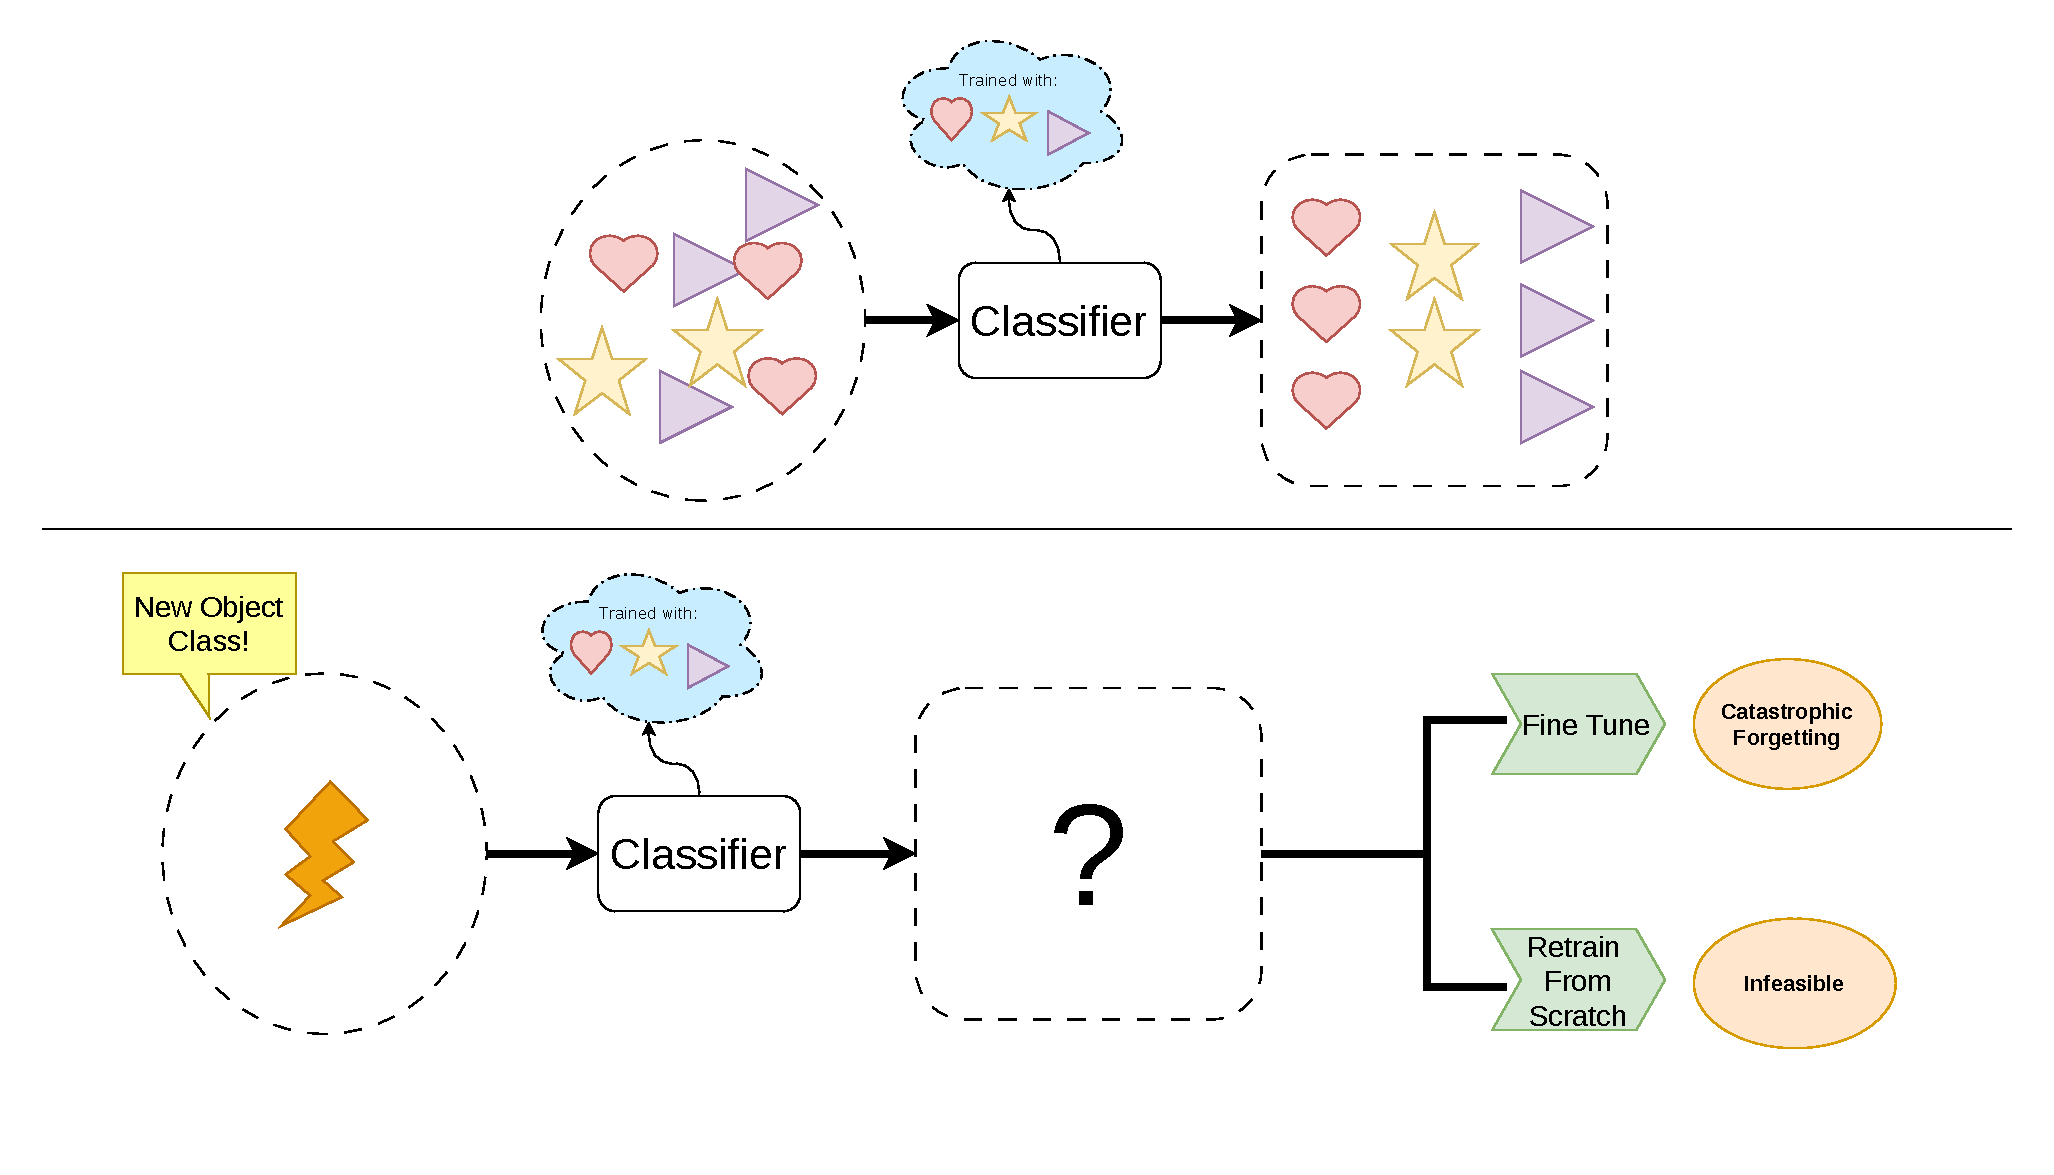
\includegraphics[width=0.8\textwidth]{imagenes/marco/Catastrophic_forgetting.pdf}
	\caption{Standard Object Classifier comparison. The upper path shows standard inference, while the lower path illustrates the dilemma when a new class is introduced: the trade-off between catastrophic forgetting via fine-tuning and the infeasibility of retraining from scratch.}
	\label{fig:catastrophic_forgetting}
\end{figure}

\subsection{Stability and Plasticity}
A central concept in continual learning is the balance between stability and plasticity. \textbf{Stability} emphasizes preserving the parameters and representations that are crucial for retaining old knowledge \cite{API}. \textbf{Plasticity}, in contrast, refers to the ability of a model to adapt rapidly to new information, ensuring that it can effectively learn novel tasks. Achieving an appropriate equilibrium between these two properties is known as the \textbf{stability–plasticity dilemma} \cite{CL}.

\subsection{Main Paradigms}
As shown in Figure \ref{fig:task_vs_class}, two principal paradigms define how continual learning problems are formulated. \textbf{Task-incremental learning (Task-IL)} assumes that the task identity is available during inference, allowing for task-specific components to be isolated \cite{task_il}. \textbf{Class-incremental learning (Class-IL)}, on the other hand, does not provide the task identity at test time, requiring the model to distinguish between all classes seen across all tasks simultaneously \cite{masana_class_il}.

\begin{figure}[htb]
	\centering
	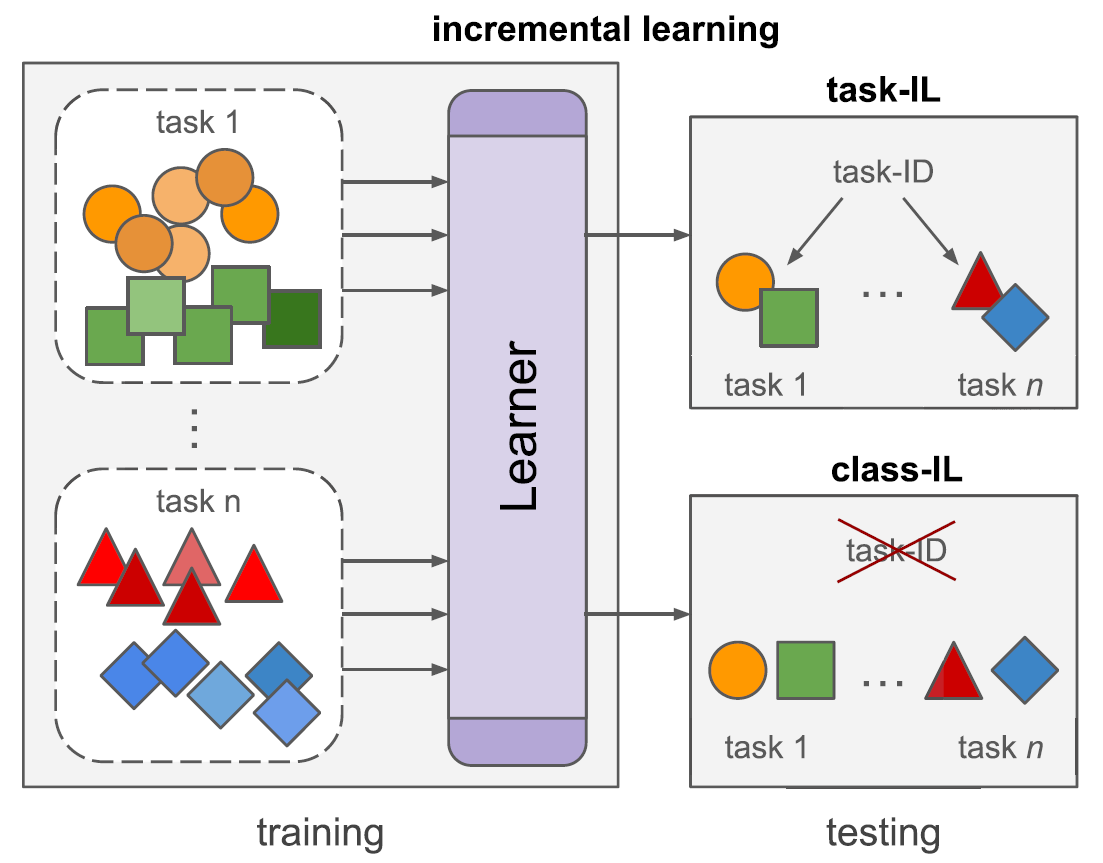
\includegraphics[width=0.5\textwidth]{imagenes/marco/CI_learning_survey_fig1.png}
	\caption{Class and Task Incremental Learning. Image taken from \cite{masana_class_il}.}
	\label{fig:task_vs_class}
\end{figure}

\subsection{Related Work in Continual Learning}

To address the stability–plasticity dilemma, we categorize continual learning strategies into five broad approaches: rehearsal, regularization, architecture-based methods, representation and prompt-based tuning, and classifier adaptation over frozen representations. Classifier adaptation—both its discriminative and analytic, prototype-based variants—is the approach most directly comparable to the framework proposed in this thesis, so it's the one we treat as the closest point of reference.

\subsubsection{Rehearsal Methods}

Rehearsal-based methods target the most direct cause of catastrophic forgetting: once training on a new task starts, there is no gradient signal left telling the model anything about what it already learned. So they mix a handful of past examples into the current task's training data—sometimes these are just the original images sitting in a small buffer, sometimes they are synthetic examples that a separate generator recreates on the fly instead of storing anything real—keeping the model reminded of the old classes even while it is busy learning the new ones. The real design question is what to keep and how to use it efficiently, since a memory buffer with no limits would defeat the whole point of a learner that has to run with limited memory and storage.

\begin{itemize}
	\item \textbf{Experience Replay (ER)} \cite{Chaudhry2019ContinualLW} is the simplest instantiation of this idea: a small episodic memory buffer retains a random or reservoir-sampled subset of past examples, which are interleaved with the current task's mini-batches so that every gradient step still receives some supervision on old classes. Its simplicity makes it a common and surprisingly strong baseline, but its effectiveness scales with buffer size, and the fixed capacity inevitably biases the retained sample toward whichever selection heuristic is used.
	
	\item \textbf{Average Gradient Episodic Memory (A-GEM)} \cite{agem} reframes the buffer's role from a source of additional gradient signal to a constraint on the optimisation trajectory itself: rather than training jointly on old and new samples, it projects the current task's gradient so that it does not increase the loss computed on a reference batch drawn from the buffer, which is considerably cheaper than the original GEM formulation while retaining most of its forgetting-mitigation benefits.
	
	\item \textbf{Dark Experience Replay (DER)} \cite{buzzega2020darkexperiencegeneralcontinual} enriches the stored exemplars with the network's own past output logits rather than only their hard labels, and distils this ``dark knowledge''---the full soft-label distribution encoding inter-class similarity structure learned at the time of storage---back into the current model. This provides a denser training signal per replayed sample than label-only rehearsal, at the cost of needing to persist and periodically re-align these logits with a model that is continually changing.
	
	\item \textbf{Generative Replay} \cite{generative_features} sidesteps the need to store raw exemplars altogether by training a generative model (or, in feature-space variants, a feature synthesiser) to reproduce samples of previously seen classes on demand. This removes the raw-data privacy liability of exemplar buffers, but transfers the difficulty elsewhere: the generator itself must be continually updated without forgetting, and any drift in the quality of its synthetic samples directly corrupts the rehearsal signal for old classes.
\end{itemize}

Across all four variants, the shared limitation is structural rather than incidental: rehearsal methods require either persistent storage of raw or compressed past data, or a generative model that is itself subject to the same forgetting dynamics it is meant to prevent, and their forgetting-mitigation quality degrades gracefully but monotonically as the buffer-to-task-count ratio shrinks over a long task stream.

\subsubsection{Regularization Methods}

Rather than revisiting old data, regularization-based methods attempt to identify, at the parameter level, which weights of the network are responsible for previously learned behaviour, and then constrain how much those specific weights are allowed to move while training on new tasks. The stability--plasticity trade-off is therefore made explicit as a per-parameter penalty: important parameters are frozen or heavily penalized for movement, while the remaining capacity of the network is left free to absorb new information.

\begin{itemize}
	\item \textbf{Elastic Weight Consolidation (EWC)} \cite{Kirkpatrick_2017} estimates parameter importance using the diagonal of the Fisher Information Matrix computed on each task, then adds a quadratic penalty to the loss that discourages movement away from the previous task's optimum in proportion to that importance. The approach is elegant and grounded in a Bayesian interpretation of sequential posterior updates, but the diagonal Fisher approximation ignores parameter interactions, and the accumulated quadratic penalties from many tasks can over-constrain the network, progressively eroding its plasticity.
	\item \textbf{Synaptic Intelligence (SI)} \cite{zenke2017continuallearningsynapticintelligence} computes an online, per-synapse importance measure by accumulating each parameter's contribution to the reduction of the loss along the entire training trajectory of a task, avoiding the need for a separate importance-estimation pass after each task and making the method considerably cheaper than EWC in practice, though it inherits a similar long-horizon rigidity problem.
	\item \textbf{Learning Without Forgetting (LwF)} \cite{li2017learningforgetting} regularises the network's function rather than its parameters directly: before training on a new task, the previous model's predictions on the new task's inputs are recorded, and a knowledge-distillation loss then penalises deviations of the updated model's outputs from these recorded soft targets. This makes LwF architecture-agnostic and exemplar-free, but its effectiveness depends on the new task's inputs being informative enough to anchor the old decision boundaries, which becomes unreliable under large domain shifts between tasks.
	\item \textbf{Adaptive Plasticity Improvement (API)} \cite{API} takes a more geometric view, using Dual Gradient Projection Memory (Dual-GPM) to identify the subspaces of parameter (or gradient) space that were important for previous tasks and enforcing that new updates proceed in directions orthogonal to them. This directly targets the stability side of the dilemma by construction, but the number of protected subspaces necessarily grows with the number of tasks, gradually shrinking the remaining free subspace available for future plasticity.
\end{itemize}

The common thread across this family is that importance estimates---whether Fisher-based, synaptic, distillation-based, or subspace-based---are necessarily approximate and computed with respect to the tasks seen so far; as the task stream lengthens, the accumulated constraints compete for a fixed parameter budget, and all four methods must trade off increasingly aggressive stability against a shrinking capacity for plasticity.

\subsubsection{Architecture-based Methods}
A third family sidesteps the stability--plasticity trade-off at the parameter level altogether by modifying the network's structure itself, either by isolating the sub-networks responsible for each task or by physically growing the network's capacity as new tasks arrive.
\begin{itemize}
	\item \textbf{Parameter Isolation} \cite{10.5555/3454287.3455512} identifies and freezes the specific parameters or sub-networks important for previous tasks---typically through pruning or learned gradient masks---so that only a designated, disjoint subset of weights remains trainable for the current task. This offers a strong, structural guarantee against forgetting for the frozen parameters, but the available free capacity shrinks monotonically as more tasks are isolated, and, in many instantiations, recovering which sub-network to use at inference time requires knowledge of the task identity.
	
	\item \textbf{Dynamic Expansion} methods take a more literal approach: instead of freezing parts of a fixed-size network, they let the network itself grow. DER~\cite{Yan2021DERDE} (Dynamically Expandable Representation, not to be confused with Dark Experience Replay above) keeps everything learned so far completely frozen and, for each new task, bolts on a brand-new trainable branch next to it; the outputs of all branches get concatenated into one large ``super-feature'', and a pruning step afterward trims away whatever redundant channels that new branch didn't really need. DEN~\cite{Yoon2017LifelongLW} (Dynamically Expandable Networks) is more conservative: rather than always adding a new branch, it first tries to fit the new task using the capacity that's already there, and only grows the network—adding new units—when the training loss shows that existing capacity genuinely isn't enough. Both approaches guarantee that old sub-networks remain untouched and hence immune to forgetting by construction, but at the cost of a parameter count, and consequently a memory and computational footprint, that grows over the lifetime of the system---an increasingly serious limitation for long task streams.
\end{itemize}

Whether through isolation or expansion, architecture-based methods trade the risk of interference for an explicit, often unbounded, growth in model complexity, and frequently still require task identity at inference to route each input to the correct sub-network---a requirement that is unavailable in the class-incremental setting studied throughout this thesis.

\subsubsection{Representation and Prompt-based Methods}
The rise of foundation models (e.g., ViTs, described in detail in Section~\ref{sec:framework:foundation_models}) opened up a different strategy altogether: instead of touching the backbone's weights at all, these methods leave it completely frozen and confine all task-specific learning to a small set of extra parameters called \emph{prompts}. Concretely, a prompt is a short sequence of learnable embedding vectors that gets prepended to, or otherwise inserted into, the sequence of patch tokens the Transformer already processes for a given image; the backbone treats these vectors exactly as it would treat any other token, so they never change a single one of the network's own weights, but they do change what the network attends to and, through that, the features it eventually outputs for that image. Since the backbone itself never changes, forgetting at the representation level cannot happen by construction; the real challenge shifts to designing prompts expressive enough to adapt the frozen features to each task, without ever telling the model which task it is currently looking at.
\begin{itemize}
	\item \textbf{Learning to Prompt (L2P)} \cite{wang2022learning} keeps a pool of learnable prompts and, for each input, picks out and combines the ones that best match it: every prompt has an associated key vector, and the input's own embedding is compared against these keys to decide which prompts to use. Because this selection is done per input rather than per task, the same shared pool can serve every task without ever needing to know which one is currently active; the trade-off is that the whole approach now depends on that matching step working correctly, and a wrong match sends the input to prompts meant for entirely different content.
	\item \textbf{Dual Prompt} \cite{wang2022dualprompt} builds on this by splitting the prompt pool into two clearly different roles: a set of fixed, shared \emph{General} prompts that capture knowledge common to all tasks, and task-specific \emph{Expert} prompts that specialize the representation for the classes belonging to one particular task. This division gives a better balance between remembering old tasks and learning new ones than L2P's single undifferentiated pool, though it still needs the same kind of key-based matching to pick out the right Expert prompt at inference time.
	\item \textbf{CODA-Prompt} \cite{Smith_2023_CVPR} does away with that hard, similarity-based matching step entirely. Instead of picking a discrete subset of prompts, it combines all of them through an attention-weighted average, so the whole prompting mechanism can be trained end-to-end together with the classifier, rather than depending on a separately tuned matching heuristic.
	\item \textbf{Advanced Prompting} extensions carry this same idea into more efficient and distributed settings: \textbf{InFLoRA} \cite{liang2024inflora} and \textbf{DOLFIN} \cite{dolfin} apply low-rank adaptation and distributed training, respectively, to cut down the parameter cost of maintaining a prompt pool, while \textbf{APT} \cite{Chen_2025_ICCV} skips prompt selection altogether by injecting key-value tokens directly into the transformer's attention layers, which also reduces the computational cost at inference time.
\end{itemize}

Across this family, freezing the backbone rules out representation-level forgetting almost by definition, but everything then depends on how well the prompt-selection mechanism works. That mechanism brings its own extra parameters and its own training difficulties, and because prompts are usually learned by backpropagating through the frozen backbone, it also adds a computational cost per task that the purely analytic methods discussed next manage to avoid entirely.

\subsubsection{Classifier Adaptation on Frozen Representations}
A complementary line of work also keeps the feature extractor frozen, just like prompt-based methods do, but skips learnable prompts entirely: the frozen embedding is simply taken as-is, and all the adaptation happens in a discriminative or metric-based classifier built directly on top of it, with no backpropagation through the backbone at all.

\begin{itemize}
	\item \textbf{SLCA} \cite{zhang2023slca} proposes a slow learner with classifier alignment for continual learning on pre-trained models: the backbone is fine-tuned with a substantially reduced learning rate to preserve its pre-trained generality, while a separate classifier head is periodically re-aligned to correct for the resulting representation drift, enabling efficient incremental learning without the full instability of end-to-end fine-tuning.
	\item \textbf{ACIL} \cite{zhuang2022acil} treats incremental learning analytically: following an initial base phase where the CNN backbone is trained via backpropagation and subsequently frozen, it projects the extracted embeddings into a higher-dimensional space via a randomized feature expansion layer with non-linear activations. A linear classifier is then updated over these expanded features using recursive regularized least-squares, which provably reproduces the joint-training closed-form solution over all observed classes without revisiting past data, ensuring absolute memorization and data privacy without exemplar storage.
	\item \textbf{FeCAM} \cite{goswami2024fecam} exploits the heterogeneity of class distributions in this exemplar-free setting by replacing the Euclidean or purely linear decision rules of the methods above with a Mahalanobis-distance-based classifier, explicitly accounting for the fact that different classes occupy differently shaped regions of the frozen embedding space.
\end{itemize}

Because the backbone is never updated, none of these methods suffers representation-level forgetting, and---unlike prompt-based methods---none of them requires backpropagation at all during incremental updates; the price is that their classifiers rely on comparatively simple statistical or geometric assumptions about the embedding space, which the next family of methods begins to make explicit.

\subsubsection{Class Prototype and Analytic Classifier Methods}
\label{sec:marco:prototype_methods}
A closely related family of methods represents each class through distances to class prototypes (first-order information), sometimes complemented by second-order statistics, and is the family most directly comparable to the framework proposed in this thesis.
\begin{itemize}
	\item \textbf{SimpleCIL} \cite{janson2022simple} performs first-session adaptation by applying parameter-efficient fine-tuning (PEFT) to the backbone only during the initial task, after which the backbone is frozen for the remainder of the stream and class prototypes are computed simply as the mean embedding of the samples belonging to each class. Its simplicity and strong empirical performance on foundation-model embeddings established that even a purely first-order, distance-to-mean classifier can be a remarkably strong baseline once the backbone is sufficiently general.
	\item \textbf{RanPAC} \cite{mcdonnell2023ranpac} improves upon this prototype-based scheme by first applying a fixed random projection followed by a non-linear activation, lifting the features into a higher-dimensional space in which classes become more linearly separable by construction (a random-feature approximation of a kernel expansion), and then accumulating second-order information through a shared, incrementally updated Gram matrix across all classes rather than per-class covariances.
	\item \textbf{FeTrIL} \cite{petit2023fetril} stores only the centroid representation of each past class rather than any raw exemplars or full covariance matrices. When a new task arrives, features of the new classes are geometrically shifted toward past class regions using the difference between past and new class centroids; the resulting pseudo-features are then used alongside real new-class features to train a linear classifier incrementally.
	\item \textbf{FeCAM} \cite{goswami2024fecam}, already introduced above, is more naturally placed in this family for its second-order treatment: it explores Mahalanobis distances instead of typical Euclidean distances, applying a Tukey power-ladder transformation to correct feature skewness before normalising each class covariance so that its diagonal entries equal one, making Mahalanobis distances comparable across classes despite never validating that the underlying feature distributions justify a Gaussian, Mahalanobis-based treatment in the first place.
\end{itemize}

Across this family, representing a class through its prototype brings real efficiency, but that efficiency comes at a representational cost: first-order methods such as SimpleCIL and FeTrIL reduce a class to a single point in the embedding space, discarding the covariance information that describes how the class's features actually spread around that point, while RanPAC and FeCAM recover richer, second-order structure without a principled probabilistic model to justify the specific distance or normalization they apply, and neither checks whether treating class covariance this way is consistent with how the class distributions actually look.

\paragraph{Summary of Limitations.}
Across all five families, the same pattern recurs: each avoids one part of the stability--plasticity trade-off only by pushing its cost elsewhere---onto a growing memory or generator, a hardening set of importance constraints, an unbounded architecture, a fragile prompt-selection mechanism, or a classifier built on first-order or heuristic statistics rather than a proper probabilistic model. None of them checks whether the Gaussian assumption behind their distance metrics actually holds in the embedding space, or ties inter-class separability directly to the accuracy that can realistically be expected.

These limitations motivate a framework that (i) avoids exemplar storage, generator training, growing architectures, and backpropagation altogether by keeping the backbone entirely frozen and updating only closed-form sufficient statistics; (ii) models each class with a full, properly normalized multivariate Gaussian density rather than a heuristic distance metric, restoring a direct probabilistic and generative interpretation; and (iii) explicitly and statistically validates the Gaussian assumption on which this generative model rests, rather than simply asserting it.

\section{Foundation Models}
\label{sec:framework:foundation_models}

Having introduced Continual Learning as the central topic of this thesis, we now turn to a different piece of background this framework depends on: foundation models, the broader category of models the representation-learning backbone belongs to, and in particular Vision Transformers and the DINOv2 architecture used as the frozen feature extractor throughout this work. Before getting into the details of these two architectures, though, it is worth stepping back and asking what a foundation model actually is, and why a model of that kind is exactly what a frozen, exemplar-free continual learner needs.

\subsection{The Foundation Model Paradigm}
\label{sec:framework:foundation_paradigm}

A \textbf{foundation model} is best understood by the role it plays rather than by any single architecture: it is a large-scale model pre-trained on vast quantities of data and subsequently adaptable to a wide range of downstream tasks with comparatively little task-specific effort. The term itself was coined by researchers at the Stanford Institute for Human-Centered AI precisely to capture this role: these models are not built for one job, but act as a common technological base on top of which many specialised applications are eventually constructed \cite{bommasani2021opportunities}.

What really changes compared to a traditional machine learning pipeline is where the effort goes. Instead of training a task-specific architecture from scratch on a carefully generated by hand dataset, foundation models split the work into two clearly separated phases. The first, \emph{pre-training at scale}, exposes the network to huge amounts of data---web text, image collections, or multimodal data, depending on the domain---often, though not always, using self-supervised objectives such as predicting masked tokens or learning contrastive or self-distilled representations, which keep manual annotation to a minimum. The network just picks up rich, general-purpose structure about whatever domain it is trained on. The second phase, \emph{downstream adaptation}, takes this pre-trained network---frozen entirely or updated only slightly---and repurposes it for a specific target task through comparatively lightweight means: linear probing, parameter-efficient fine-tuning, or even zero-shot prompting, without ever retraining the backbone from scratch.


This two-phase recipe works across pretty much any type of data, largely because most foundation models, whatever they are trained on, share the same underlying architecture: the Transformer. In language, this gives rise to models such as GPT, Llama, and Gemini, which learn how words and phrases relate to each other well enough to support reasoning, translation, and text generation. In vision, the same recipe produces Vision Transformers and segmentation models such as the Segment Anything Model (SAM) \cite{kirillov2023segment}, which build detailed spatial and visual representations that carry over to detection, segmentation, and classification tasks. And across different types of data at once, systems such as CLIP or GPT-4o map images, text, and audio into a single shared space, letting them reason across all of them together.

\subsection{Vision Transformers}

Within this landscape, Vision Transformers are the specific architecture this thesis builds on. As introduced in Section~\ref{sec:framework:cv}, the Transformer---originally developed for Natural Language Processing---changed visual recognition by relying on self-attention \cite{AttentionIsAllYouNeed}, a mechanism that lets every element of the input attend directly to every other element, and this challenged the long-standing dominance of Convolutional Neural Networks (CNNs) \cite{CNN} in Computer Vision.

A Vision Transformer (ViT) adapts this architecture to images by treating them as a sequence of discrete tokens, the same kind of input a Transformer would otherwise expect from a sentence of words. As illustrated in Figure \ref{fig:ViTArchitecture}, this is done through a specific pipeline:

\begin{itemize}
	\item \textbf{Patch Partitioning:} The input image is divided into a grid of fixed-size patches, each of which becomes one token in the sequence.
	\item \textbf{Linear Projection:} Each patch is flattened into a vector and projected into an embedding space, giving every token a numerical representation the network can operate on.
	\item \textbf{Positional Encoding:} Since self-attention treats the sequence as an unordered set, it has no inherent notion of where each patch sat in the original image; a learnable positional embedding is therefore added to each patch embedding to encode its location in the grid.
	\item \textbf{Transformer Encoder:} The resulting sequence of position-aware patch tokens is processed by several stacked layers of multi-head self-attention and feed-forward blocks, which allow the model to relate tokens from anywhere in the image to one another and build up a global representation.
\end{itemize}

\begin{figure}[htb]
	\centering
	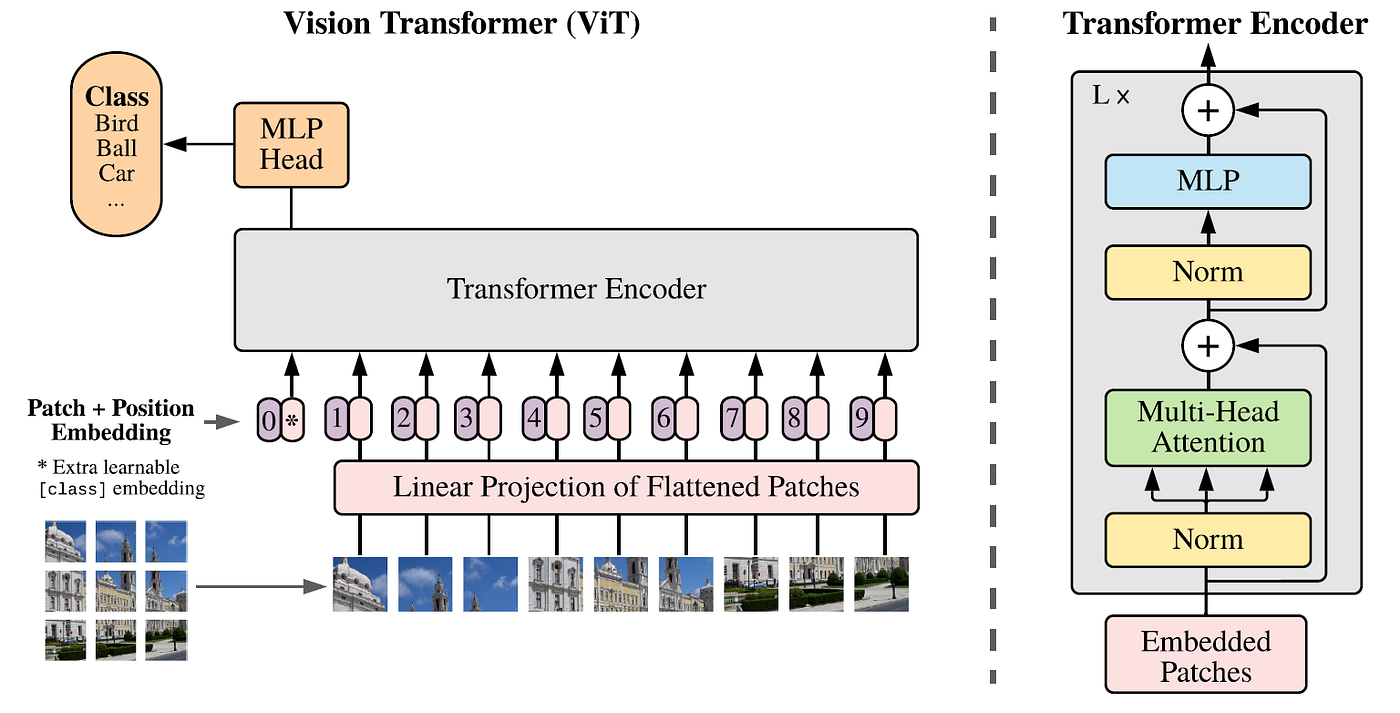
\includegraphics[width=0.7\textwidth]{imagenes/marco/ViT.png}
	\caption{Vision Transformer (ViT) architecture overview. The model processes an image as a sequence of patches through a standard Transformer encoder. Image taken from \cite{AnImageIsWorth}.}
	\label{fig:ViTArchitecture}
\end{figure}

\subsubsection{Object Classification and Representative Power}
The original ViT was designed and evaluated primarily on Object Classification, the task introduced in Section~\ref{sec:framework:cv} that also serves as the setting for the Continual Learning problem studied in this thesis. By attending over the full sequence of patch tokens rather than a local receptive field, ViTs have shown they can match or exceed CNN performance on this task, particularly when pre-trained on the kind of large-scale datasets described below.

\subsubsection{Self-Supervised Advancements: DINOv2}

Most vision datasets are still built around labels assigned by hand, but recent work has shifted toward foundation models trained via self-supervised learning instead, following the same general pre-training paradigm described earlier in this chapter: no human-provided labels are used at all. A leading example of this approach is \textbf{DINOv2} \cite{oquab2024dinov}, which produces visual features that are robust and general enough to perform well ``out of the box,'' both at the level of whole-image descriptions and at the level of individual patch tokens.

DINOv2 is built around a \textbf{Student-Teacher self-distillation} framework, extending earlier work on DINO \cite{DINO} and iBOT \cite{ibot}. Two networks of identical architecture are trained in parallel: a \textit{Student} network $g_{\theta_s}$, whose weights are updated by gradient descent as usual, and a \textit{Teacher} network $g_{\theta_t}$, which is never trained directly and instead tracks the student as an Exponential Moving Average (EMA) of its weights $\theta_s$:

\begin{equation}
	\theta_t \leftarrow \lambda \theta_t + (1 - \lambda) \theta_s
\end{equation}

where $\lambda \in [0, 1]$ is a smoothing parameter controlling how slowly the teacher follows the student. During training, the framework optimizes two complementary objectives to learn both global and fine-grained spatial representations:

\begin{itemize}
	\item \textbf{Image-Level Loss (DINO):} The student is fed both global and local crops of the same image, while the teacher only ever processes global views. The student is trained to match the teacher's output distribution over a set of learned prototype vectors, an online \textit{Sinkhorn-Knopp centering} step keeping this matching balanced so that the representations do not collapse to a single trivial solution.
	\item \textbf{Patch-Level Loss (iBOT):} To force the model to capture dense, local structure rather than only a global summary, a subset of the student's input patch tokens are masked out. The student must then reconstruct the teacher's corresponding patch-level features, computed from the same image without any masking.
	\item \textbf{KoLeo Regularization:} To keep the resulting embeddings spread out across the feature space rather than collapsing into a narrow region, DINOv2 adds a term based on the Kozachenko-Leonenko (KoLeo) differential entropy estimator, which penalizes feature vectors for lying too close to their nearest neighbor within a training batch:
	\begin{equation}
		\mathcal{L}_{\text{KoLeo}} = -\frac{1}{n}\sum_{i=1}^{n} \log \left( \min_{j \neq i} \| \vec{x}_i - \vec{x}_j \|_2 \right)
	\end{equation}
	where $\vec{x}_i$ is the $\ell_2$-normalized feature vector of the $i$-th image in a batch of size $n$.
\end{itemize}
